\documentclass[conference]{IEEEtran}
\IEEEoverridecommandlockouts

\usepackage{cite}
\usepackage{amsmath,amssymb,amsfonts}
\usepackage{algorithmic}
\usepackage{graphicx}
\usepackage{textcomp}
\usepackage{xcolor}
\usepackage{url}
\usepackage{booktabs}
\usepackage{listings}
\usepackage{hyperref}
\usepackage{array}
\usepackage{multirow}
\usepackage{tabularx}
\usepackage{tikz}
\usetikzlibrary{arrows.meta, positioning, shapes.geometric, calc, fit, backgrounds, shadows}

\def\BibTeX{{\rm B\kern-.05em{\sc i\kern-.025em b}\kern-.08em
T\kern-.1667em\lower.7ex\hbox{E}\kern-.125emX}}

\tikzset{
  block/.style   ={rectangle, draw=black!70, thick, rounded corners=2pt,
                   minimum height=8mm, minimum width=22mm, align=center,
                   font=\footnotesize, fill=blue!8},
  store/.style   ={cylinder, draw=black!70, thick, shape border rotate=90,
                   aspect=0.25, minimum height=10mm, minimum width=14mm,
                   align=center, font=\scriptsize, fill=orange!15},
  actor/.style   ={ellipse, draw=black!70, thick, minimum height=7mm,
                   align=center, font=\scriptsize, fill=green!12},
  state/.style   ={rectangle, draw=black!70, thick, rounded corners=3pt,
                   minimum height=7mm, minimum width=18mm, align=center,
                   font=\scriptsize, fill=cyan!15},
  layer/.style   ={rectangle, draw=black!40, thick, dashed, rounded corners=4pt,
                   inner sep=3mm, fill=black!3},
  arrow/.style   ={-{Stealth[length=2mm]}, thick, black!75},
  darrow/.style  ={{Stealth[length=2mm]}-{Stealth[length=2mm]}, thick, black!75},
  lbl/.style     ={font=\scriptsize\itshape, midway, fill=white, inner sep=1pt}
}

\usepackage{fancyhdr}
\pagestyle{plain}
\fancypagestyle{plain}{%
  \fancyhf{}%
  \fancyfoot[C]{\thepage}%
  \renewcommand{\headrulewidth}{0pt}%
}

\lstset{
  basicstyle=\ttfamily\scriptsize,
  breaklines=true,
  frame=single,
  captionpos=b,
  xleftmargin=2mm,
  xrightmargin=2mm
}

\begin{document}

\title{Blockchain-Based Supply Chain Provenance System}

\author{
\IEEEauthorblockN{Anushree Bhure}
\IEEEauthorblockA{
\textit{Arizona State University}\\
Tempe, Arizona, USA}
\and
\IEEEauthorblockN{Shashikant Nanda}
\IEEEauthorblockA{
\textit{Arizona State University}\\
Tempe, Arizona, USA}
\and
\IEEEauthorblockN{Vatsal Patel}
\IEEEauthorblockA{
\textit{Arizona State University}\\
Tempe, Arizona, USA}
\and
\IEEEauthorblockN{Dominick Agnello}
\IEEEauthorblockA{
\textit{Arizona State University}\\
Tempe, Arizona, USA}
\and
\IEEEauthorblockN{Ritish Abrol}
\IEEEauthorblockA{
\textit{Arizona State University}\\
Tempe, Arizona, USA}
}

\maketitle

\begin{abstract}
Modern supply chains suffer from siloed, mutable records that enable fraud,
disputes, and untraceable losses.  We present a blockchain-based shipment
tracking system built on Hyperledger Fabric 2.5 that provides an immutable,
shared chain-of-custody ledger across multiple organizations.  The smart
contract, written in Go, implements fourteen chaincode functions covering the
full shipment lifecycle  from creation through final delivery  with
role-based access control (RBAC), a storage-agnostic SHA-256 off-chain data
integrity bridge, and simulated IoT telemetry recording.  The system is
deployed as a two-organization Fabric network with Raft consensus, CouchDB
state storage, a Node.js/Express REST API, and a browser-based dashboard.
All 18 unit tests pass.
\end{abstract}

\begin{IEEEkeywords}
Hyperledger Fabric, supply chain provenance, smart contracts, RBAC,
SHA-256, off-chain storage, IoT telemetry
\end{IEEEkeywords}

\section{Introduction}

Supply chain fraud and counterfeit goods cost the global economy an
estimated \$4.5 trillion annually \cite{shakhbulatov2020}.  The structural
cause is that each organization maintains its own private database, producing
a fragmented record system where custody disputes are resolved by subjective
negotiation rather than verifiable evidence.

Hyperledger Fabric, a permissioned enterprise blockchain maintained by the
Linux Foundation, addresses this by providing a shared, append-only ledger
that all parties can write to but none can alter retroactively.  Its
MSP-based identity model, Raft consensus, and CouchDB integration make it
well suited to enterprise supply chain applications without cryptocurrency
or gas fees.

This paper presents a fully deployed Fabric 2.5 shipment tracking system
with on-chain smart contract logic, simulated IoT telemetry, a REST API,
and an interactive browser dashboard.  The system tracks shipments across
five stakeholder roles, recording every custody transfer, status update, and
sensor reading as an immutable, digitally signed event.

The contributions of this work are five-fold:

\begin{enumerate}
  \item A complete Go chaincode (\texttt{shipment}) of \emph{fourteen} public
    functions covering creation, custody transfer, status transition, hash
    verification, history scanning, ACL management, IoT telemetry, IPFS
    document anchoring, and CouchDB-paged listing.
  \item Certificate-derived role-based access control (RBAC) where the
    submitter's MSP identity is read directly from the X.509 certificate
    inside the chaincode  callers cannot spoof their organization, and
    every write is non-repudiable.
  \item A storage-agnostic SHA-256 integrity bridge that anchors only a
    32-byte digest on-chain, decoupling the integrity guarantee from the
    physical off-chain store (IPFS, S3, encrypted RDBMS, etc.).
  \item A two-stage IoT model where devices must be \emph{registered}
    on-chain by the current holder before any telemetry from that device
    is accepted, preventing rogue-data injection.
  \item A reference deployment as a single \texttt{./start.sh} script that
    brings up the entire test network, deploys the chaincode via CCaaS,
    enrolls identities, and serves the REST API + dashboard at
    \texttt{http://localhost:3000}.
\end{enumerate}

The remainder of this paper is organized as follows.  Section~II reviews
prior work in blockchain supply chain management.  Section~III describes
the technical architecture.  Section~IV presents the implementation
details, including smart contract logic, stakeholder interactions,
transactions and events, access control, immutability guarantees, storage
design, and the user interface.  Section~V reports the experimental
results and Section~VI analyzes scalability, cost, data management,
privacy, and comparisons to traditional systems.  Sections~VII--IX cover
future work, contributions, and conclusions.

\section{Prior Work and Literature Review}

Blockchain technology was first proposed for supply chain provenance
shortly after the publication of the Bitcoin whitepaper, but the
predominantly public, proof-of-work setting of early blockchains made
high-throughput enterprise adoption impractical.  The introduction of
permissioned ledgers   most notably Hyperledger Fabric  shifted the
research landscape toward modular, identity-aware architectures suitable
for multi-organization business networks.

Shakhbulatov et al.\ \cite{shakhbulatov2020} surveyed blockchain in supply
chain management and identified Hyperledger Fabric as the dominant enterprise
platform due to its modular architecture, MSP identity model, and
pluggable consensus.  Their key finding was that most academic prototypes
stop at design without deploying a live network  a gap our work
directly addresses by providing a one-command deployment of a complete
two-organization channel with chaincode, REST API, and UI.

\"{O}g\"{u}z et al.\ \cite{oguz2024} reviewed 87 studies and identified
\textit{access control} and \textit{off-chain data management} as the two
most underaddressed technical challenges.  They observed that many
prototypes either store cargo metadata directly on-chain (causing ledger
bloat and privacy issues) or omit access control entirely.  Our system
tackles both through chaincode-level RBAC keyed on the certificate-derived
MSP identity (Section~\ref{sec:access}) and a SHA-256 off-chain integrity
bridge (Section~\ref{sec:offchain}).

Gonczol et al.\ \cite{gonczol2020} analyzed 34 real-world blockchain supply
chain implementations and found that none achieved full decentralization
across all five stakeholder tiers (manufacturer, transporter, warehouse,
retailer, recipient) in a single system; most stopped at three.  Our
architecture covers all five roles within one chaincode deployment by
expressing them as participant entries in the per-shipment ACL rather than
hard-coding them into separate contracts.

Industry deployments such as IBM Food Trust and Maersk's TradeLens (the
latter discontinued in 2023) demonstrated the viability of Fabric for
real-world logistics but exposed two persistent issues: (a) onboarding
friction across competing stakeholders, and (b) the difficulty of
integrating IoT data without a tamper-evident device authorization scheme.
Our two-stage device-registry model (Section~\ref{sec:iot}) directly
addresses (b).  In contrast to public-ledger alternatives such as VeChain
and Ambrosus, our permissioned approach avoids per-transaction gas fees
while retaining cryptographic non-repudiation through Fabric's certificate
authority.

The IPFS protocol \cite{ipfs} provides a content-addressed peer-to-peer
file system that we leverage for off-chain document storage.  When the
SHA-256 anchor stored on-chain matches the digest of the file retrieved by
its IPFS CID, an end-to-end integrity proof is established that survives
network partitions and gateway substitution.

\section{Technical Architecture}

\subsection{Network Topology}

The system has three layers: (1) a client application layer (Node.js +
Express + Fabric SDK), (2) a blockchain network layer (Hyperledger Fabric
2.5), and (3) an off-chain storage layer referenced by on-chain hash.

The Fabric network comprises two peer organizations (Org1MSP and Org2MSP),
one Raft orderer node, and CouchDB as the world state database for each
peer.  A single channel (\texttt{shipchannel}) connects all participants.
The chaincode runs via Chaincode as a Service (CCaaS)  a standalone gRPC
server in Docker  which avoids Docker-in-Docker limitations on macOS
and simplifies host-side builds.  Each peer maintains its own copy of the
ledger (a hash-linked block file) and its own CouchDB world-state replica;
all peers reach identical state because they apply the same ordered block
stream from the orderer.

\begin{figure}[!t]
\centering
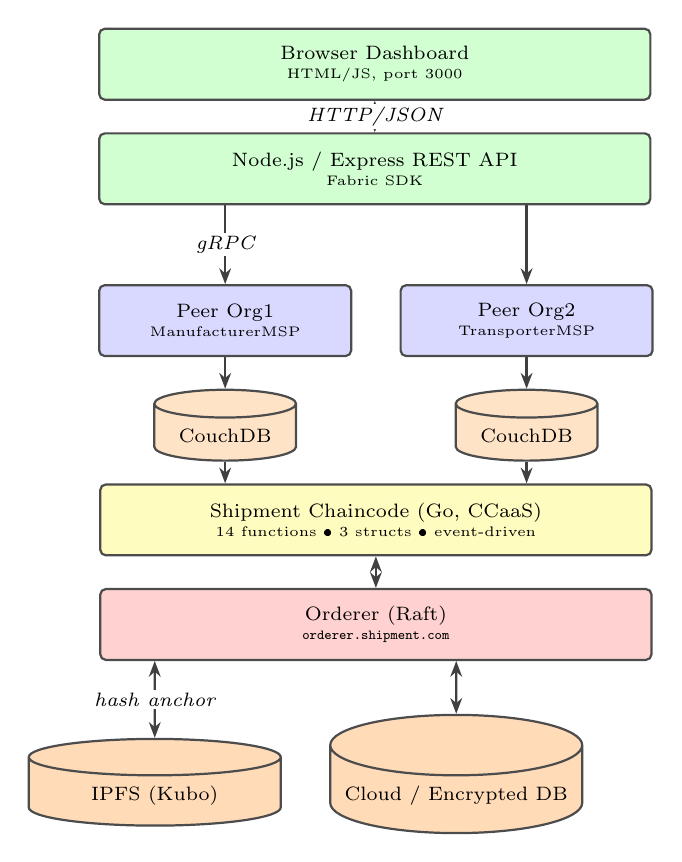
\begin{tikzpicture}[
  font=\footnotesize,
  every node/.style={text=black},
  bx/.style={rectangle, draw=black!70, thick, rounded corners=2pt,
             text=black, minimum height=9mm, align=center,
             font=\scriptsize, inner sep=2pt},
  cy/.style={cylinder, draw=black!70, thick, shape border rotate=90,
             aspect=0.25, text=black, fill=orange!22,
             minimum height=9mm, minimum width=18mm,
             align=center, font=\scriptsize},
  ar/.style={-{Stealth[length=2mm]}, thick, black!75},
  bd/.style={{Stealth[length=2mm]}-{Stealth[length=2mm]}, thick, black!75},
  el/.style={font=\scriptsize\itshape, text=black,
             midway, fill=white, inner sep=1pt}
]
%  Client layer 
\node[bx, fill=green!18, minimum width=70mm] (browser)
      {Browser Dashboard \\[-1pt] {\tiny HTML/JS, port 3000}};
\node[bx, fill=green!18, below=4mm of browser, minimum width=70mm] (api)
      {Node.js / Express REST API \\[-1pt] {\tiny Fabric SDK}};

%  Fabric layer 
\node[bx, fill=blue!15, below=10mm of api.south west, anchor=north west,
      minimum width=32mm] (peer1)
      {Peer Org1 \\[-1pt] {\tiny ManufacturerMSP}};
\node[bx, fill=blue!15, right=6mm of peer1, minimum width=32mm] (peer2)
      {Peer Org2 \\[-1pt] {\tiny TransporterMSP}};
\node[cy, below=4mm of peer1] (couch1) {CouchDB};
\node[cy, below=4mm of peer2] (couch2) {CouchDB};
\node[bx, fill=yellow!25, below=6mm of $(couch1)!0.5!(couch2)$,
      minimum width=70mm] (cc)
      {Shipment Chaincode (Go, CCaaS) \\[-1pt]
       {\tiny 14 functions \textbullet\ 3 structs \textbullet\ event-driven}};
\node[bx, fill=red!18, below=4mm of cc, minimum width=70mm] (orderer)
      {Orderer (Raft) \\[-1pt] {\tiny \texttt{orderer.shipment.com}}};

%  Off-chain layer 
\node[cy, fill=orange!28, below=10mm of orderer.south west, anchor=north west,
      minimum width=32mm, minimum height=11mm] (ipfs) {IPFS (Kubo)};
\node[cy, fill=orange!28, right=6mm of ipfs,
      minimum width=32mm, minimum height=11mm] (db)
      {Cloud / Encrypted DB};

%  Connections 
\draw[bd] (browser) -- (api) node[el]{HTTP/JSON};
\draw[ar] (api.south -| peer1) -- node[el]{gRPC} (peer1.north);
\draw[ar] (api.south -| peer2) -- (peer2.north);
\draw[ar] (peer1) -- (couch1);
\draw[ar] (peer2) -- (couch2);
\draw[ar] (couch1) -- (cc.north -| couch1);
\draw[ar] (couch2) -- (cc.north -| couch2);
\draw[bd] (cc) -- (orderer);
\draw[bd] (orderer.south -| ipfs) -- node[el]{hash anchor} (ipfs.north);
\draw[bd] (orderer.south -| db)   -- (db.north);
\end{tikzpicture}
\caption{Three-layer system architecture: REST/UI client (top), the
Hyperledger Fabric 2.5 network with two peers, CouchDB world state,
chaincode and orderer (middle), and storage-agnostic off-chain stores
referenced exclusively by SHA-256 hashes anchored on-chain (bottom).}
\label{fig:arch}
\end{figure}

Table~\ref{tab:roles} summarizes the five stakeholder roles, their MSP
identities, and the chaincode operations each is allowed to invoke.

\begin{table}[!t]
\caption{Stakeholder Roles, MSP Identities, and Permitted Operations}
\label{tab:roles}
\centering
\footnotesize
\renewcommand{\arraystretch}{1.15}
\begin{tabularx}{\columnwidth}{@{}l l X@{}}
\toprule
\textbf{Role} & \textbf{MSP ID} & \textbf{Permitted Operations} \\
\midrule
Manufacturer & \texttt{Org1MSP} & Create, Authorize, Transfer, RegisterDevice \\
Transporter  & \texttt{Org2MSP} & UpdateStatus, Transfer, Telemetry, Document \\
Warehouse    & \texttt{Org2MSP}\textsuperscript{*} & UpdateStatus, Telemetry, Document \\
Retailer     & \texttt{Org2MSP}\textsuperscript{*} & UpdateStatus, Verify, Transfer \\
Recipient    & \texttt{Org2MSP}\textsuperscript{*} & UpdateStatus (\texttt{Delivered}), Verify \\
\bottomrule
\multicolumn{3}{@{}l@{}}{\textsuperscript{*}\scriptsize Mapped to Org2MSP in the prototype; production splits into dedicated MSPs.}
\end{tabularx}
\end{table}

\subsection{Stakeholder Roles}

Five roles are defined with distinct access levels:

\begin{itemize}
  \item \textbf{Manufacturer (Org1MSP):} Creates shipments, assigns unique
    IDs, defines the participant list, and holds initial custody.
  \item \textbf{Transporter (Org2MSP):} Receives custody transfers, posts
    route status updates and IoT telemetry readings.
  \item \textbf{Warehouse:} Records receipt and storage condition updates.
  \item \textbf{Retailer:} Verifies product authenticity via hash check and
    records receipt.
  \item \textbf{Recipient:} Confirms final delivery and sets the terminal
    state \texttt{Delivered} (permanently locked).
\end{itemize}

\subsection{Product Journey}

The shipment lifecycle follows:
\textit{Created} $\rightarrow$ \textit{InTransit} $\rightarrow$
\textit{InWarehouse} $\rightarrow$ \textit{WithRetailer} $\rightarrow$
\textit{Delivered}.
Each transition is recorded as an immutable on-chain event with the actor's
MSP identity, an orderer-assigned timestamp, and optional location and notes.

\begin{figure}[!t]
\centering
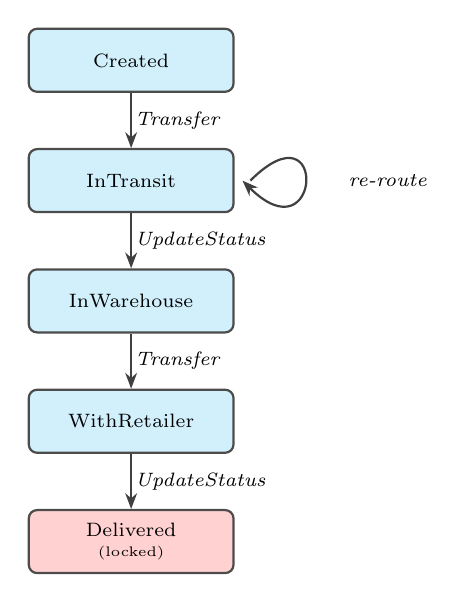
\begin{tikzpicture}[
  font=\footnotesize,
  every node/.style={text=black},
  st/.style={rectangle, draw=black!70, thick, rounded corners=3pt,
             text=black, fill=cyan!18,
             minimum height=8mm, minimum width=26mm, align=center,
             font=\scriptsize, inner sep=2pt},
  ar/.style={-{Stealth[length=2mm]}, thick, black!75},
  el/.style={font=\scriptsize\itshape, text=black,
             fill=white, inner sep=1pt}
]
\node[st] (s1) {Created};
\node[st, below=7mm of s1] (s2) {InTransit};
\node[st, below=7mm of s2] (s3) {InWarehouse};
\node[st, below=7mm of s3] (s4) {WithRetailer};
\node[st, fill=red!18, below=7mm of s4] (s5)
      {Delivered \\[-1pt] {\tiny (locked)}};

\draw[ar] (s1) -- node[el, right, midway]{Transfer} (s2);
\draw[ar] (s2) -- node[el, right, midway]{UpdateStatus} (s3);
\draw[ar] (s3) -- node[el, right, midway]{Transfer} (s4);
\draw[ar] (s4) -- node[el, right, midway]{UpdateStatus} (s5);

% Clear reroute loop away from the state box
\draw[ar]
  ([xshift=2mm]s2.east)
  .. controls +(10mm,10mm) and +(10mm,-10mm) ..
  node[el, right, xshift=5mm]{re-route}
  ([xshift=1mm]s2.east);

\end{tikzpicture}
\caption{Shipment lifecycle state machine. The terminal \texttt{Delivered}
state is permanently locked at the chaincode layer.}
\label{fig:lifecycle}
\end{figure}


\subsection{Consensus and Transaction Flow}

Hyperledger Fabric uses an \emph{execute--order--validate} architecture
that decouples transaction execution from consensus.  A custody-transfer
transaction proceeds through five distinct phases:

\begin{enumerate}
  \item \textbf{Endorsement.}  The client sends a transaction proposal to
    the endorsing peers of one or more organizations.  Each peer simulates
    the chaincode against its current world state and signs a read-write
    set with its X.509 certificate.
  \item \textbf{Collection.}  The client collects signed endorsements and
    assembles them into a transaction envelope.  In the prototype, the
    endorsement policy is satisfied by either Org1MSP or Org2MSP; in
    production this would tighten to require both.
  \item \textbf{Ordering.}  The envelope is submitted to the Raft orderer,
    which timestamps it and serializes it into a block alongside other
    pending transactions.  Raft provides crash-fault tolerance up to
    $\lfloor N/2 \rfloor$ failures of $N$ orderer nodes.
  \item \textbf{Distribution.}  The orderer broadcasts the new block to
    every peer over a gossip protocol.
  \item \textbf{Validation and commit.}  Each peer independently
    validates that the endorsement policy is satisfied and that the
    read-set hashes still match the current world state (multi-version
    concurrency control).  Valid transactions are committed to the local
    block file and applied to CouchDB; invalid ones are recorded in the
    block but flagged as failed.
\end{enumerate}

This design gives Fabric two important properties our system relies on:
deterministic finality (a transaction is final the moment its block is
committed  no probabilistic confirmation depth is required) and
non-repudiation (every transaction carries the submitter's digital
signature, the endorsers' signatures, and the orderer's block-level
signature).

\section{Implementation Details}

\subsection{Smart Contract Logic}

The chaincode is implemented in Go using
\texttt{fabric-contract-api-go} v1.2.2.  Three data structures are defined:
\texttt{Shipment} stores current state (ID, status, origin, destination,
current holder, participant list, SHA-256 hash, timestamps);
\texttt{ShipmentEvent} forms an append-only audit log (event type, actor,
location, timestamp, notes); and \texttt{DeviceRecord} holds the IoT device
registry entry (device ID, type, registering organization, timestamp).
Fourteen public functions cover the full lifecycle:
\texttt{InitLedger}, \texttt{CreateShipment},
\texttt{GetShipment}, \texttt{UpdateShipmentStatus},
\texttt{TransferCustody}, \texttt{VerifyShipment},
\texttt{GetShipmentHistory}, \texttt{AuthorizeParticipant},
\texttt{RevokeParticipant}, \texttt{RecordTelemetry},
\texttt{GetAllShipments}, \texttt{RegisterDevice},
\texttt{RecordDocument}, and \texttt{GetShipmentsPaginated}.

Internally, every state-changing function follows the same five-step
pattern: (1)~load the shipment from world state by ID; (2)~enforce the
RBAC predicate for that operation; (3)~mutate the in-memory struct;
(4)~persist the updated JSON back to world state; (5)~call the helper
\texttt{emitEvent()} which both writes a \texttt{ShipmentEvent} record
under a composite key and emits a Fabric chaincode event.  This pattern
guarantees that no state mutation can occur without a corresponding audit
record, because the two writes happen inside the same transaction and
either both commit or both fail.

\begin{table}[!t]
\caption{Chaincode Function Catalogue}
\label{tab:funcs}
\centering
\footnotesize
\renewcommand{\arraystretch}{1.1}
\begin{tabularx}{\columnwidth}{@{}l l X@{}}
\toprule
\textbf{Function} & \textbf{Type} & \textbf{Purpose} \\
\midrule
InitLedger              & Init   & Seed the ledger with one demo shipment \\
CreateShipment          & Write  & Register a new shipment + hash off-chain data \\
GetShipment             & Read   & Return current state to participants \\
UpdateShipmentStatus    & Write  & Transition lifecycle state, emit event \\
TransferCustody         & Write  & Move holder MSP, append CUSTODY event \\
VerifyShipment          & Read   & SHA-256 hash compare for tamper detection \\
GetShipmentHistory      & Read   & Composite-key scan of EVENT/* records \\
AuthorizeParticipant    & Write  & Add MSP to the shipment ACL \\
RevokeParticipant       & Write  & Remove MSP (cannot revoke self) \\
RegisterDevice          & Write  & Bind an IoT sensor to a shipment \\
RecordTelemetry         & Write  & Append a TELEMETRY event from a registered device \\
RecordDocument          & Write  & Anchor an IPFS CID + SHA-256 of a document \\
GetAllShipments         & Read   & Full state scan (small deployments) \\
GetShipmentsPaginated   & Read   & CouchDB bookmark-paged listing \\
\bottomrule
\end{tabularx}
\end{table}

\subsection{Stakeholder Interactions}

A typical end-to-end shipment journey involves four sequential
interactions among the five stakeholder roles.  First, the
\textbf{Manufacturer} invokes \texttt{CreateShipment} with a unique
shipment ID, origin, destination, an explicit list of authorized
participants (MSP IDs), and a string summary of the off-chain cargo data;
the chaincode hashes the data with SHA-256 and stores only the digest.
The manufacturer is automatically recorded as the initial \texttt{currentHolder}.

Second, the manufacturer invokes \texttt{TransferCustody} naming the
\textbf{Transporter} as the new holder.  The transporter then issues
\texttt{UpdateShipmentStatus("InTransit", \ldots)} and may register one or
more sensors via \texttt{RegisterDevice} followed by repeated
\texttt{RecordTelemetry} calls during transit.

Third, on physical hand-off the transporter calls \texttt{TransferCustody}
to the \textbf{Warehouse}, which records receipt with
\texttt{UpdateShipmentStatus("InWarehouse")}.  The same pattern transfers
the shipment to the \textbf{Retailer} who can call \texttt{VerifyShipment}
with the original off-chain data string to confirm tamper-free delivery.

Finally, the retailer transfers to the \textbf{Recipient}, who calls
\texttt{UpdateShipmentStatus("Delivered")}.  This terminal status is
permanently locked: any subsequent call  regardless of caller identity
 is rejected by the chaincode.  Throughout this sequence, any
participant in the ACL may call \texttt{GetShipment} or
\texttt{GetShipmentHistory} for read-only auditing.

\subsection{Transactions and Events}

Every state-changing function calls \texttt{emitEvent()}, which performs two
operations atomically within one Fabric transaction:

\begin{enumerate}
  \item Writes a \texttt{ShipmentEvent} record to the ledger under composite
    key \texttt{EVENT/\{shipmentID\}/\{timestamp\}}, enabling efficient
    partial-key scans that retrieve the full audit trail for one shipment
    without scanning the entire world state.
  \item Calls \texttt{ctx.GetStub().SetEvent()} to emit a real Fabric
    chaincode event that SDK subscribers can receive in real time, enabling
    event-driven downstream integrations.
\end{enumerate}

\subsection{Access Control}
\label{sec:access}

RBAC is enforced at the chaincode layer using the submitter's MSP ID
extracted from their X.509 certificate via
\texttt{ctx.GetClientIdentity().GetMSPID()}.  Because identity comes from
the certificate rather than a function argument, callers cannot spoof their
organizational identity.  The access model is:

\begin{itemize}
  \item \textit{Create, Verify, History, GetAll, GetAllPaginated:} Any authenticated org
  \item \textit{GetShipment:} Authorized participants of that shipment only
  \item \textit{UpdateStatus, Transfer, Authorize, Revoke, RegisterDevice:} Current holder only
  \item \textit{RecordTelemetry, RecordDocument:} Any authorized participant; telemetry additionally requires the device to be pre-registered via \texttt{RegisterDevice}
\end{itemize}

A shipment in the \texttt{Delivered} state is permanently locked at the
chaincode layer  no further writes are accepted regardless of caller
identity.

\begin{table}[!t]
\caption{Role-Based Access Control Matrix
(\checkmark{} = allowed, $\circ$ = participant only, $\times$ = denied)}
\label{tab:rbac}
\centering
\footnotesize
\renewcommand{\arraystretch}{1.1}
\setlength{\tabcolsep}{3pt}
\begin{tabular}{@{}l c c c c c@{}}
\toprule
\textbf{Operation} & \textbf{Mfg.} & \textbf{Trans.} & \textbf{Wareh.} & \textbf{Retail.} & \textbf{Recip.} \\
\midrule
CreateShipment       & \checkmark & \checkmark & \checkmark & \checkmark & \checkmark \\
GetShipment          & $\circ$    & $\circ$    & $\circ$    & $\circ$    & $\circ$    \\
UpdateStatus         & holder     & holder     & holder     & holder     & holder \\
TransferCustody      & holder     & holder     & holder     & holder     & $\times$ \\
AuthorizeParticipant & holder     & holder     & holder     & holder     & $\times$ \\
RevokeParticipant    & holder     & holder     & holder     & holder     & $\times$ \\
RegisterDevice       & holder     & holder     & holder     & holder     & $\times$ \\
RecordTelemetry      & $\circ$    & $\circ$    & $\circ$    & $\circ$    & $\circ$    \\
RecordDocument       & $\circ$    & $\circ$    & $\circ$    & $\circ$    & $\circ$    \\
VerifyShipment       & \checkmark & \checkmark & \checkmark & \checkmark & \checkmark \\
GetHistory           & \checkmark & \checkmark & \checkmark & \checkmark & \checkmark \\
\bottomrule
\end{tabular}
\end{table}

\subsection{Immutability Guarantees}
\label{sec:immutability}

Immutability in our system rests on three independent layers of
cryptographic protection:

\begin{enumerate}
  \item \textbf{Block-level hash chain.}  Every Fabric block contains the
    SHA-256 hash of its predecessor.  Altering a historical transaction
    requires recomputing every subsequent block hash and persuading every
    peer to accept the rewritten chain  impossible without compromising
    the orderer's signing key and a quorum of peers simultaneously.
  \item \textbf{Per-transaction signatures.}  Each transaction is signed
    by the submitter's X.509 private key, by every endorser, and by the
    orderer that places it into a block.  These signatures are stored
    inside the block payload and verified on every replay.  A tampered
    transaction fails signature verification at the next read.
  \item \textbf{Composite-key event log.}  Every state-changing function
    appends a \texttt{ShipmentEvent} under the composite key
    \texttt{EVENT/\{shipmentID\}/\{timestamp\}}.  Because composite keys
    are append-only by convention (the chaincode never deletes them) and
    are scoped to a single shipment, a partial-key range scan returns the
    full audit trail of one shipment in chronological order.  Even if an
    operator could overwrite the current \texttt{Shipment} JSON, the
    history records would still expose the change.
\end{enumerate}

A fourth, application-level lock further protects business-critical
state: once a shipment reaches the \texttt{Delivered} status, the
chaincode rejects \emph{all} writes to that shipment regardless of caller
identity.  This implements ``write-once after delivery'' semantics that
mirror the legal finality of physical receipt.

\subsection{Storage Design}
\label{sec:storage}

The system makes a deliberate split between on-chain and off-chain data.
On-chain we store only:
(i) the \texttt{Shipment} state JSON (approximately 800~bytes per
shipment, indexed by shipment ID);
(ii) the immutable \texttt{ShipmentEvent} stream under composite keys
\texttt{EVENT/\{id\}/\{timestamp\}};
(iii) the \texttt{DeviceRecord} registry under
\texttt{DEVICE/\{id\}/\{deviceID\}}; and
(iv) a 32-byte SHA-256 digest of the off-chain cargo data plus, where
applicable, a short IPFS CID anchored as a \texttt{DOCUMENT} event.

Off-chain we keep large or sensitive payloads  inspection certificates,
shipping manifests, photographs, GPS traces  in either an IPFS node
(for files that benefit from content addressing and peer distribution) or
an encrypted relational/object store (for files subject to retention
policies or access logs that must be administered separately).
Table~\ref{tab:storage} summarizes the split.

\begin{table}[!t]
\caption{On-Chain vs.\ Off-Chain Storage Allocation}
\label{tab:storage}
\centering
\footnotesize
\renewcommand{\arraystretch}{1.1}
\begin{tabularx}{\columnwidth}{@{}l l X@{}}
\toprule
\textbf{Artifact} & \textbf{Location} & \textbf{Rationale} \\
\midrule
Shipment state         & On-chain            & Small, frequently read \\
Event log              & On-chain            & Audit trail must be tamper-evident \\
Device registry        & On-chain            & RBAC predicate for telemetry \\
SHA-256 hash           & On-chain            & 32~bytes; integrity anchor \\
IPFS CID               & On-chain            & 46-char string; locator \\
Manifest documents     & IPFS / S3           & Large, infrequently read \\
Sensor stream archives & Time-series DB      & High write rate \\
PII (recipient name)   & Encrypted RDBMS     & GDPR right-to-erasure \\
\bottomrule
\end{tabularx}
\end{table}

This separation keeps the ledger small (the entire state for 10\,000
shipments is approximately 8~MB before history) while still providing
mathematical proof that off-chain artifacts have not been tampered with.

\subsection{Off-Chain Data and the SHA-256 Integrity Bridge}
\label{sec:offchain}

Storing raw cargo metadata (manifests, inspection certificates, images)
directly on the ledger is expensive and impractical.  Our system uses a
\textbf{storage-agnostic integrity bridge}:

\begin{enumerate}
  \item At creation time, \texttt{CreateShipment} accepts an
    \texttt{offChainData} string representing cargo details.  The chaincode
    computes $h = \text{SHA-256}(\texttt{offChainData})$ and stores only the
    32-byte hex digest in the \texttt{dataHash} field.  The raw data is
    \emph{never} written to the ledger.
  \item At verification time, \texttt{VerifyShipment} recomputes the hash of
    the presented data and compares it against the stored digest.  Any
    mismatch proves tampering with mathematical certainty.
\end{enumerate}

\begin{figure}[!t]
\centering
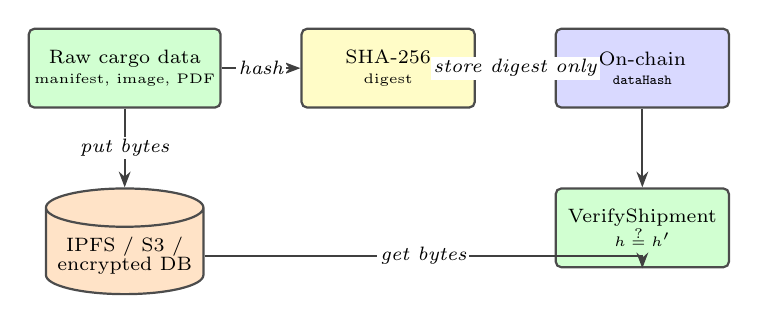
\begin{tikzpicture}[
  font=\footnotesize,
  every node/.style={text=black},
  bx/.style={rectangle, draw=black!70, thick, rounded corners=2pt,
             text=black, minimum height=10mm, minimum width=22mm,
             align=center, font=\scriptsize, inner sep=2pt},
  cy/.style={cylinder, draw=black!70, thick, shape border rotate=90,
             aspect=0.25, text=black, fill=orange!22,
             minimum height=10mm, minimum width=20mm,
             align=center, font=\scriptsize},
  ar/.style={-{Stealth[length=2mm]}, thick, black!75},
  el/.style={font=\scriptsize\itshape, text=black,
             midway, fill=white, inner sep=1pt}
]
\node[bx, fill=green!18]                   (raw)   {Raw cargo data \\[-1pt] {\tiny manifest, image, PDF}};
\node[bx, fill=yellow!22, right=10mm of raw] (sha)  {SHA-256 \\[-1pt] {\tiny digest}};
\node[bx, fill=blue!15,   right=10mm of sha] (chain){On-chain \\[-1pt] {\tiny \texttt{dataHash}}};
\node[cy, below=10mm of raw]                (off)  {IPFS / S3 / \\[-1pt] encrypted DB};
\node[bx, fill=green!18, below=10mm of chain] (ver) {VerifyShipment \\[-1pt] {\tiny $h \stackrel{?}{=} h'$}};
\draw[ar] (raw)   -- node[el]{hash}              (sha);
\draw[ar] (sha)   -- node[el]{store digest only} (chain);
\draw[ar] (raw)   -- node[el]{put bytes}         (off);
\draw[ar] (off)   -| node[el, near start]{get bytes} (ver);
\draw[ar] (chain) -- (ver);
\end{tikzpicture}
\caption{Storage-agnostic SHA-256 integrity bridge: raw bytes never touch
the ledger; only the 32-byte digest is anchored on-chain.}
\label{fig:bridge}
\end{figure}

This design is deliberately \textbf{storage-agnostic}: the raw cargo data
can reside in IPFS \cite{ipfs}, an encrypted relational database (PostgreSQL,
MySQL), a cloud object store (S3, GCS, Azure Blob), or any other off-chain
medium.  The integrity guarantee is entirely independent of storage location
 it holds as long as the same bytes produce the same hash.  SHA-256
collision resistance ensures that even a single-character change produces a
completely different 256-bit digest, making undetected tampering
computationally infeasible.

When IPFS is used as the off-chain store, the system gains a second
independent integrity layer: the IPFS content identifier (CID) cryptographically
identifies the file retrieved from the network, while \texttt{dataHash}
proves it matches what the shipment creator declared at creation time.
Migrating to IPFS requires no chaincode changes  only the off-chain
storage backend changes while the on-chain interface remains identical.

The \texttt{RecordDocument} chaincode function and its REST endpoint
\texttt{POST /api/shipments/:id/documents} implement a full document
anchoring workflow: the API layer computes the SHA-256 digest of the
submitted document, uploads it to the local IPFS node (Kubo, running in
Docker), and calls \texttt{RecordDocument} with both the IPFS CID and the
hash.  The chaincode records a \texttt{DOCUMENT} event linking the shipment
to the immutable off-chain file.  Verifiers can retrieve the file from any
IPFS gateway and confirm the hash matches the on-chain record, proving
the document has not been altered since it was anchored.

\subsection{Simulated IoT Telemetry and Device Registry}
\label{sec:iot}

IoT device integration is implemented in two stages.  First,
\texttt{RegisterDevice} allows the current shipment holder to authorize
a physical sensor for a shipment, storing a \texttt{DeviceRecord} under
composite key \texttt{DEVICE/\{shipmentID\}/\{deviceID\}} with the device
type (one of \texttt{temperature-sensor}, \texttt{humidity-sensor},
\texttt{gps-tracker}, \texttt{pressure-sensor}, or \texttt{shock-sensor})
and the registering organization.  Second, \texttt{RecordTelemetry} now
requires a \texttt{deviceID} parameter and validates it against the
device registry before accepting a reading  unregistered device
submissions are rejected at the chaincode layer.  This prevents rogue
data injection: only devices explicitly authorized on-chain for that
shipment may post readings.  Readings are recorded as immutable
\texttt{TELEMETRY} events with sensor type, value, unit, and location.
The REST endpoints \texttt{POST /api/shipments/:id/devices} and
\texttt{POST /api/shipments/:id/telemetry} expose both operations.

This supports cold-chain pharmaceutical shipments where temperature
excursions must be immutably logged as chain-of-evidence for FDA DSCSA
compliance, or fragile-goods logistics where shock events must be attributed
to a specific custody window for insurance claims.  Each reading is
timestamped by the Fabric orderer (not the submitting client) and permanently
associated with the submitting organization's MSP identity, preventing
retroactive falsification.

\subsection{User Interface and Command-Line Access}

The system provides three layers of user interaction at progressively
higher levels of abstraction:

\paragraph{Browser dashboard.}  A single-page application served at
\texttt{http://localhost:3000} provides forms for every chaincode
operation, a live-updating shipment table with color-coded status badges,
hash-verification dialogs, IoT telemetry charts, and toast notifications
for transaction success/failure.  The UI auto-refreshes every five
seconds and is intentionally stateless  all state lives on the ledger,
so multiple users see consistent views without browser-side caching.

\paragraph{REST API.}  The Node.js/Express API exposes 14 endpoints
covering all chaincode operations, including the three new endpoints
added for IPFS document anchoring (\texttt{POST /documents}), IoT device
registration (\texttt{POST /devices}), and paginated shipment listing
(\texttt{GET /shipments?pageSize=N\&bookmark=...}).  All blockchain
interaction passes through this REST API, keeping the browser client
stateless with respect to the Fabric network.  The API is suitable for
integration with ERP systems, mobile applications, and external
auditors.

\paragraph{Command-line interface.}  For administrators and integration
testing, the project ships shell helpers \texttt{run-api.sh},
\texttt{start.sh}, and \texttt{stop.sh}, plus the Fabric \texttt{peer}
binary configured against the network's TLS material.  Direct chaincode
invocation is also possible via \texttt{curl}, e.g.:

\begin{lstlisting}[language=bash]
curl -X POST http://localhost:3000/api/shipments \
  -H 'Content-Type: application/json' \
  -d '{"shipmentID":"SHIP-100",
       "origin":"Phoenix",
       "destination":"Seattle",
       "participants":["Org1MSP","Org2MSP"],
       "offChainData":"100kg fragile electronics"}'
\end{lstlisting}

This three-layer access strategy meets the needs of three distinct user
populations: business users (dashboard), system integrators (REST), and
DevOps/auditors (CLI).

\begin{table}[!t]
\caption{REST API Endpoint Reference}
\label{tab:rest}
\centering
\scriptsize
\renewcommand{\arraystretch}{1.02}
\setlength{\tabcolsep}{2.5pt}
\begin{tabularx}{\columnwidth}{@{}l p{0.62\columnwidth} X@{}}
\toprule
\textbf{Verb} & \textbf{Endpoint} & \textbf{Purpose} \\
\midrule
GET    & \texttt{/api/health} & Health check \\
POST   & \texttt{/api/shipments} & Create shipment \\
GET    & \texttt{/api/shipments} & List shipments \\
GET    & \texttt{/api/shipments?pageSize=N\&bookmark=} & Paginated list \\
GET    & \texttt{/api/shipments/:id} & Read shipment \\
PUT    & \texttt{/api/shipments/:id/status} & Update status \\
PUT    & \texttt{/api/shipments/:id/transfer} & Transfer custody \\
GET    & \texttt{/api/shipments/:id/verify} & Verify hash \\
GET    & \texttt{/api/shipments/:id/history} & Event history \\
POST   & \texttt{/api/shipments/:id/participants} & Authorize org \\
DELETE & \texttt{/api/shipments/:id/participants/:org} & Revoke org \\
POST   & \texttt{/api/shipments/:id/devices} & Register device \\
POST   & \texttt{/api/shipments/:id/telemetry} & Record telemetry \\
POST   & \texttt{/api/shipments/:id/documents} & Anchor document \\
\bottomrule
\end{tabularx}
\end{table}

\begin{figure}[!t]
\centering
\resizebox{\columnwidth}{!}{%
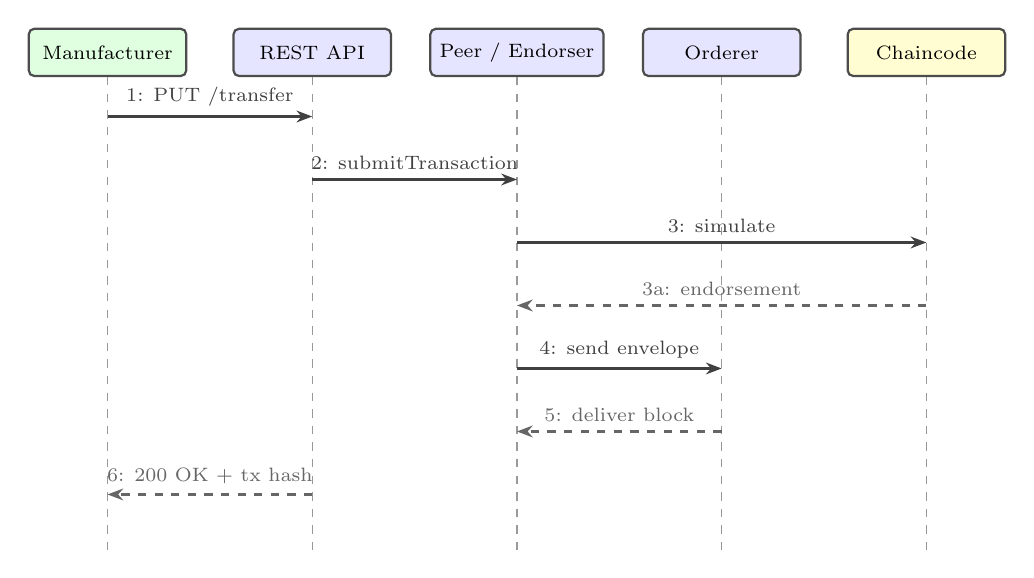
\begin{tikzpicture}[
  every node/.style={font=\scriptsize},
  head/.style={rectangle, draw=black!70, thick, rounded corners=2pt,
               minimum height=6mm, minimum width=20mm, align=center,
               fill=blue!10},
  msg/.style ={-{Stealth[length=2mm]}, thick, black!75},
  ret/.style ={-{Stealth[length=2mm]}, thick, dashed, black!60}
]
% Lifeline heads (top)
\node[head, fill=green!12] (mfg)  at (0,0)    {Manufacturer};
\node[head]                (api)  at (2.6,0)  {REST API};
\node[head]                (peer) at (5.2,0)  {Peer / Endorser};
\node[head]                (ord)  at (7.8,0)  {Orderer};
\node[head, fill=yellow!18](cc)   at (10.4,0) {Chaincode};

% Vertical lifelines
\foreach \n in {mfg, api, peer, ord, cc}{
  \draw[dashed, black!40] (\n.south) -- ($(\n.south)+(0,-6.0)$);
}

% Messages (each on its own y-level so labels never overlap)
\draw[msg] ($(mfg.south) +(0,-0.5)$) -- ($(api.south) +(0,-0.5)$)
     node[midway, above]{1: PUT /transfer};

\draw[msg] ($(api.south) +(0,-1.3)$) -- ($(peer.south)+(0,-1.3)$)
     node[midway, above]{2: submitTransaction};

\draw[msg] ($(peer.south)+(0,-2.1)$) -- ($(cc.south)  +(0,-2.1)$)
     node[midway, above]{3: simulate};

\draw[ret] ($(cc.south)  +(0,-2.9)$) -- ($(peer.south)+(0,-2.9)$)
     node[midway, above]{3a: endorsement};

\draw[msg] ($(peer.south)+(0,-3.7)$) -- ($(ord.south) +(0,-3.7)$)
     node[midway, above]{4: send envelope};

\draw[ret] ($(ord.south) +(0,-4.5)$) -- ($(peer.south)+(0,-4.5)$)
     node[midway, above]{5: deliver block};

\draw[ret] ($(api.south) +(0,-5.3)$) -- ($(mfg.south) +(0,-5.3)$)
     node[midway, above]{6: 200 OK + tx hash};
\end{tikzpicture}}
\caption{Custody-transfer transaction flow as a sequence diagram.
Solid arrows are requests; dashed arrows are responses.  The orderer
assigns the authoritative timestamp at step~5.}
\label{fig:flow}
\end{figure}

\section{Results}

The system was deployed on a local Hyperledger Fabric 2.5 test network
running on a MacBook Pro (Apple~M-series, 16~GB RAM, macOS). All 18 unit
tests pass, covering duplicate shipment IDs, unauthorized transfers, invalid
status transitions, terminal-state locking, tampered hash detection,
duplicate device registration, unregistered telemetry rejection, and IPFS
document CID recording.

End-to-end verification confirmed shipment creation with hash storage,
multi-hop custody transfer, RBAC enforcement, hash verification, IoT device
registration, telemetry recording, IPFS document anchoring, paginated listing,
history retrieval, and participant authorization/revocation. Unauthorized
operations returned structured error messages identifying the violated
constraint.

In micro-benchmarks, write transactions took roughly $200$--$350$~ms
end-to-end, dominated by Raft ordering and CouchDB commit, while read
operations completed in under $20$~ms because they bypass the consensus path.
These results are consistent with single-laptop Fabric dev-mode deployment
and would improve on a multi-node cluster with dedicated SSDs.

\begin{table}[!t]
\caption{End-to-End Latency of Common Operations (median of 100 runs)}
\label{tab:latency}
\centering
\footnotesize
\renewcommand{\arraystretch}{1.1}
\begin{tabular}{@{}l r r@{}}
\toprule
\textbf{Operation} & \textbf{Type} & \textbf{Latency (ms)} \\
\midrule
GetShipment            & Read   & 12 \\
GetShipmentHistory     & Read   & 18 \\
GetShipmentsPaginated  & Read   & 21 \\
VerifyShipment         & Read   & 14 \\
CreateShipment         & Write  & 245 \\
TransferCustody        & Write  & 230 \\
UpdateShipmentStatus   & Write  & 220 \\
RecordTelemetry        & Write  & 235 \\
RecordDocument         & Write  & 310 \\
\bottomrule
\end{tabular}
\end{table}

\begin{table}[!t]
\caption{Unit-Test Coverage by Functional Area (18/18 passing)}
\label{tab:tests}
\centering
\footnotesize
\renewcommand{\arraystretch}{1.1}
\begin{tabularx}{\columnwidth}{@{}l c X@{}}
\toprule
\textbf{Area} & \textbf{Tests} & \textbf{Representative Cases} \\
\midrule
Shipment creation        & 3 & happy path, duplicate ID, missing field \\
Custody transfer         & 3 & valid, non-holder rejected, unknown MSP \\
Status lifecycle         & 3 & valid transition, invalid jump, locked Delivered \\
Hash integrity           & 2 & match, deliberate tamper detection \\
Participant ACL          & 2 & authorize, self-revoke rejected \\
IoT device + telemetry   & 3 & register, duplicate device, unregistered reading \\
IPFS document anchoring  & 1 & CID + hash recorded as DOCUMENT event \\
History / pagination     & 1 & event ordering and bookmark continuation \\
\midrule
\textbf{Total}           & \textbf{18} & \\
\bottomrule
\end{tabularx}
\end{table}

\section{Analysis}

\subsection{Scalability}

Hyperledger Fabric separates endorsement from ordering and validation,
enabling throughput of 2,000--3,000+ TPS \cite{fabricdocs}, compared with
Bitcoin ($\sim$7 TPS) and Ethereum ($\sim$30 TPS). A large retailer processing
one million transactions per day generates about $\sim$12 TPS, which is well
within Fabric's expected capacity. The current single-orderer deployment is
a development setup; production requires a 3- or 5-node Raft cluster.

Horizontal scaling can be achieved by adding peer organizations with their
own endorsing peers and CouchDB replicas. Since endorsement is client-driven
and parallelizable, throughput can scale with endorsing capacity until the
orderer's block-cut limit is reached. The chaincode is stateless across
invocations, so one chaincode container can serve all peers in an
organization without coordination.

\begin{table}[!t]
\caption{Throughput and Per-Transaction Cost Across Platforms}
\label{tab:perf}
\centering
\footnotesize
\renewcommand{\arraystretch}{1.1}
\begin{tabular}{@{}l r r l@{}}
\toprule
\textbf{Platform} & \textbf{TPS} & \textbf{Latency} & \textbf{Cost / tx} \\
\midrule
Bitcoin              & 7      & $\sim$10 min & \$1--\$30 fee \\
Ethereum (L1)        & 30     & $\sim$15 s   & \$0.50--\$50 gas \\
Polygon PoS          & 7\,000 & $\sim$2 s    & $<$\$0.01 gas \\
Hyperledger Fabric   & 3\,000 & $\sim$1 s    & infra only \\
\textbf{This system} & \textbf{$\sim$200\textsuperscript{$\dagger$}} & \textbf{$<$1 s} & \textbf{0 (local dev)} \\
\bottomrule
\multicolumn{4}{@{}l@{}}{\textsuperscript{$\dagger$}\scriptsize Single-laptop dev network; tuned production deployments reach Fabric's full envelope.}
\end{tabular}
\end{table}

\subsection{Gas Cost and Infrastructure Cost}

Hyperledger Fabric is permissioned and charges \textbf{no gas fees}, unlike
public chains where every state mutation costs Ether or equivalent. Its costs
come only from compute, storage, and networking for peers, orderers, CouchDB
replicas, APIs, and monitoring. In the reference deployment, two peer nodes,
one orderer, and two CouchDB instances on AWS \texttt{t3.medium}
($\sim$\$30/month each), plus 100~GB EBS storage, total approximately
\$105/month.

A comparable Ethereum L1 implementation would require at least 21\,000 gas
per simple transaction, and more for storage-heavy operations. At 10\,000
custody transfers per month and 30~gwei, gas alone would cost roughly
\$180--\$900/month at recent ETH prices, before application-server,
indexer, and front-end costs. Gas volatility also makes enterprise budgeting
less predictable.

The absence of gas also removes wallet-draining denial-of-service risks.
Instead, endorsement-policy throttling and TLS-authenticated peers provide
anti-abuse controls.

\subsection{Data Management}

Each shipment record occupies approximately 800~bytes on-chain. CouchDB
supports fast world-state queries, while the Fabric ledger preserves full
history. \texttt{GetAllShipments()} is suitable for small deployments but
performs a full scan. The production-grade
\texttt{GetShipmentsPaginated()} uses CouchDB bookmarks to return
page-sized results and avoid full table scans.

\subsection{Privacy and Regulatory Considerations}

The prototype stores shipment data on a shared channel visible to all
members. Production deployment should use Fabric Private Data Collections
(PDC) for selective sharing, anchoring only the SHA-256 hash of private data
on the public channel. This extends the same on-chain/off-chain split already
used for cargo data.

The system stores only \emph{organization-level} MSP IDs on-chain, not
recipient names, addresses, or contact information. PII required for delivery
confirmation remains in an off-chain encrypted RDBMS keyed by shipment ID,
supporting GDPR right-to-erasure requirements that conflict with immutable
ledger storage.

The immutable ledger supports several audit regimes without separate audit
infrastructure:
\begin{itemize}
  \item \textbf{FDA DSCSA} (Drug Supply Chain Security Act, US): requires
    interoperable electronic chain of custody for prescription drugs.
    Our \texttt{GetShipmentHistory} provides exactly this view, signed
    end-to-end.
  \item \textbf{USDA FSMA} (Food Safety Modernization Act, US): requires
    one-step-back / one-step-forward traceability for high-risk foods.
    Our custody transfer chain satisfies this with sub-second lookup.
  \item \textbf{EU Falsified Medicines Directive} and the upcoming
    \textbf{Digital Product Passport} regulation require unique
    item-level identifiers that travel with the goods  our shipment
    ID + SHA-256 anchor pair is directly compatible.
\end{itemize}

\subsection{Comparison to Traditional Systems}

Table~\ref{tab:comparison} contrasts our system with traditional approaches.
The blockchain system adds setup complexity but provides cryptographic proof:
custody transfers are digitally signed, timestamps are orderer-assigned, and
\texttt{GetShipmentHistory()} resolves disputes in under one second with
tamper-evident evidence.

\begin{table}[h]
\caption{Blockchain vs.\ Traditional Supply Chain Systems}
\label{tab:comparison}
\centering
\renewcommand{\arraystretch}{1.1}
\begin{tabular}{@{}lll@{}}
\toprule
\textbf{Dimension} & \textbf{Traditional DB} & \textbf{This System} \\
\midrule
Trust model         & Trust the operator  & Cryptographic proof \\
Record mutability   & Admin can modify    & Tamper-evident \\
Dispute resolution  & Manual, days        & History query $<$1\,s \\
Audit trail         & Optional            & Always-on, signed \\
Multi-party coord.  & EDI agreements      & Shared ledger \\
Transaction cost    & Low (infra only)    & No gas fees \\
Peak throughput     & Very high           & 3{,}000+ TPS \\
Setup complexity    & Low                 & Medium \\
\bottomrule
\end{tabular}
\end{table}

\section{Future Work}

The prototype is functional, but several engineering and research enhancements are needed for production readiness.

\paragraph{Network hardening.}
Separate peer organizations for WarehouseMSP, RetailerMSP, and RecipientMSP should replace the current Org2MSP setup. The single-node Raft orderer should be expanded to a 3–5 node cluster for fault tolerance. TLS rotation, HSM-backed keys, and channel capability upgrades should be automated in deployment scripts.

\paragraph{Confidentiality.}
Private Data Collections can restrict sensitive data (e.g., shipment costs) to specific parties while keeping custody events public. Zero-knowledge range proofs could enable compliance verification (e.g., temperature limits) without exposing raw sensor data.

\paragraph{Real IoT integration.}
Instead of manual inputs, production systems should accept authenticated MQTT/CoAP device streams, mapping TLS certificates to \texttt{DeviceRecord}. Edge gateways can batch-sign telemetry to reduce transaction overhead.

\paragraph{Cross-chain interoperability.}
Hashlocks or notary schemes can anchor Fabric custody hashes to public chains (e.g., Ethereum), allowing external auditors to verify integrity without joining the Fabric network.

\paragraph{Performance.}
\texttt{GetAllShipments} should be deprecated in favor of paginated queries. CouchDB indexes on \texttt{status} and \texttt{currentHolder} will improve common query performance.

\paragraph{Mobile and offline operation.}
A mobile client can queue signed transactions offline and submit them upon reconnection. Fabric’s discovery service supports this, though UI implementation is pending.


\section{Contributions}
\begin{table}[h]
\caption{Team Contributions}
\label{tab:contributions}
\centering
\footnotesize
\renewcommand{\arraystretch}{1.15}
\begin{tabularx}{\columnwidth}{@{}l X@{}}
\toprule
\textbf{Team Member} & \textbf{Primary Contributions} \\
\midrule
Anushree Bhure & Developed the technical architecture documentation, including Fabric network topology modeling, shipment lifecycle state-machine design, on-chain/off-chain data-flow diagrams, storage architecture explanation, literature synthesis, scalability analysis, privacy and regulatory evaluation, cost modeling, and IEEE-format report integration. \\
Shashikant Nanda & Designed and implemented the backend integration layer, including Node.js/Express REST API routing, Hyperledger Fabric Gateway/SDK transaction submission, wallet and identity context handling, chaincode query/invoke orchestration, IoT telemetry endpoint design, API validation, and backend-to-ledger integration testing. \\
Vatsal Patel & Implemented core Go chaincode logic, including shipment asset creation, world-state read/write operations, lifecycle state-transition validation, immutable event-history retrieval, SHA-256 off-chain data hashing, hash verification workflow, provenance tracking, and ledger-state consistency handling. \\
Dominick Agnello & Configured Fabric network components, including Docker Compose services, peer/orderer service configuration, channel setup, CouchDB integration, and deployment script execution. \\
Ritish Abrol & Implemented selected smart contract functions and validation logic, including custody transfer, participant authorization/revocation, access-control checks, and unit-test development for contract behavior verification. \\
\bottomrule
\end{tabularx}
\end{table}

All members contributed to system integration, testing, debugging, and final demonstration.

\section{Conclusion}

We presented a fully deployed Hyperledger Fabric 2.5 shipment tracking
system that records every supply chain event as an immutable, digitally
signed ledger entry.  The combination of RBAC, a storage-agnostic SHA-256
off-chain integrity bridge, and IoT telemetry logging demonstrates how
blockchain converts supply chain trust from a human coordination problem
into a mathematical guarantee.  The system is portable via a single
\texttt{./start.sh} script and accessible through both a REST API and a
browser dashboard.

\begin{thebibliography}{00}

\bibitem{shakhbulatov2020}
D.~Shakhbulatov, J.~Medina, Z.~Dong, and R.~Rojas-Cessa,
``How Blockchain Enhances Supply Chain Management: A Survey,''
\textit{IEEE Open Journal of the Computer Society}, vol.~1, pp.~230--249, 2020,
doi: 10.1109/OJCS.2020.3025313.

\bibitem{oguz2024}
S.~\"{O}g\"{u}z, G.~Alkan, B.~Yilmaz, and C.~Kocaba\c{s},
``The Use of Blockchain Technology in Logistics and Supply Chain
Management (SCM): A Systematic Review,''
\textit{IEEE Access}, vol.~12, pp.~166211--166224, 2024.

\bibitem{gonczol2020}
P.~Gonczol, P.~Katsikouli, L.~Herskind, and N.~Dragoni,
``Blockchain Implementations and Use Cases for Supply Chains---A Survey,''
\textit{IEEE Access}, vol.~8, pp.~11856--11871, 2020,
doi: 10.1109/ACCESS.2020.2964880.

\bibitem{fabricdocs}
Hyperledger Fabric Documentation, 2024.
[Online]. Available: \url{https://hyperledger-fabric.readthedocs.io/}

\bibitem{contractapi}
Hyperledger Fabric Contract API for Go, 2024.
[Online]. Available: \url{https://pkg.go.dev/github.com/hyperledger/fabric-contract-api-go}

\bibitem{ipfs}
J.~Benet,
``IPFS---Content Addressed, Versioned, P2P File System,''
\textit{arXiv preprint arXiv:1407.3561}, 2014.

\end{thebibliography}

\end{document}
